\documentclass{beamer}
% Naloga 1.3.1: Za dokument uporabite razred `beamer'.
% Ne dodajajte nastavitve za velikost pisave, kot je bila v datoteki `5-prosojnice.tex`.
\usepackage{tikz}
\usetikzlibrary{math}

\usepackage{pgfplots}
\usepgfplotslibrary{external}
% Naloga 1.3.2: vključite paket `predavanja'.
\usepackage{predavanja}

% Naloga 1.3.3: definirajte okolji `definicija' in `izrek'.
% Namig: z iskanjem po datotekah (Ctrl+Shift+F oz. Cmd+Shift+F) 
% poiščite niz `{definicija}' ali niz `{izrek}'.
\newtheorem{definicija}{Definicija}
\newtheorem{izrek}{Izrek}

\begin{document}

% Naloga 1.3.4: pripravite naslovno stran z vsebino:
\title {Matematični izrazi in uporaba paketa \texttt{beamer}}
\subtitle{\emph{Matematičnih} nalog ni treba reševati!}
\institute{Fakulteta za matematiko in fiziko}
\date{}
% Zgornje podatke nastavite z ukazi kot v dokumentih razreda `article`.
% Več o tem, kako se naredi naslovno stran, si preberite na naslovu na naslovu:
% https://www.overleaf.com/learn/latex/Beamer
% To stran preberite do vključno razdelka "Creating a table of contents".
% Ukaz `\titlepage` deluje podobno kot ukaz `\maketitle`, ki ste ga že srečali.
\frame{\titlepage}


% Naloga 1.3.5: pripravite kazalo vsebine.
% 1. Naslov prosojnice, s kazalom vsebine naj bo "Kratek pregled"
% 2. S pomožnim parametrom `pausesections' (v oglatih oklepajih) 
%    določite, da naj se kazalo vsebine odkriva postopoma.
%    Poglejte, kako deluje ta ukaz.
% 3. Ker ni videti preveč lepo, pomožni parameter zakomentirajte.

\begin{frame}
    \frametitle{Kratek pregled}
    \tableofcontents%[pausesections]
\end{frame}

\section{Paket \texttt{beamer}}
%  Naslov prosojnice lahko naredimo tudi z dodatnim parametrom okolja `frame`.
\begin{frame}{Posebnosti prosojnic}
	% Naloga 2.3.1:
	% Dodajte ukaze, ki bodo poskrbeli, da se bo prosojnica odkrivala postopoma,
	% tako kot v datoteki prosojnice-resitev.pdf

	 Za prosojnice je značilna uporaba okolja \texttt{frame},
	s katerim definiramo posamezno prosojnico,\pause
	%
	 postopno odkrivanje prosojnic,\pause
	%
	 ter nekateri drugi ukazi, ki jih najdemo v paketu \texttt{beamer}.\pause
	%
	\begin{exampleblock}{Primer}
		Verjetno ste že opazili, da za naslovno prosojnico niste uporabili
		ukaza \texttt{maketitle}, ampak ukaz \texttt{titlepage}.
	\end{exampleblock}
\end{frame}

\begin{frame}{Poudarjeni bloki}
	% Naloga 2.3.2:
	% Oblikujte poudarjena bloka z opombo in opozorilom.
		\begin{block}{Opomba}
			Okolja za poudarjene bloke so \texttt{block}, \texttt{exampleblock} in \texttt{alertblock}.
		\end{block}
		
		\begin{alertblock}{Pozor!}
			Začetek poudarjenega bloka (ukaz \texttt{begin}) vedno sprejme 
		dva parametra: okolje in naslov bloka.
		Drugi parameter (za naslov) je lahko prazen.
		\end{alertblock}
		 

\end{frame}

\begin{frame}{Tudi v predstavitvah lahko pišemo izreke in dokaze}
	% Naloga 2.3.2:
	% Oblikujte okolje itemize, tako da se bo njegova vsebina postopoma odkrivala.
	% Ne smete uporabiti ukaza `pause'.
	% Beseda `največje' naj bo poudarjena šele na četrti podprosojnici.

	\begin{izrek}
	   Praštevil je neskončno mnogo.
	\end{izrek}
	\begin{proof}
	   Denimo, da je praštevil končno mnogo.
	   	% S pomožnim parametrom <+-> lahko določimo, da se bodo 
		% elementi naštevanja odkrivali postopoma.
	   \begin{itemize}[<+->]
		  \item Naj bo $p$ \alert<4>{največje} praštevilo. 
		  \item Naj bo $q$ produkt števil $1$, $2$, \ldots, $p$. 
		  \item Število $q+1$ ni deljivo z nobenim praštevilom, torej je $q+1$ praštevilo. 
		  \item To je protislovje, saj je $q+1>p$. \qedhere
	   \end{itemize}
	\end{proof}
 \end{frame}
 

\section{Paketa \texttt{amsmath} in \texttt{amsfonts}}
\begin{frame}{Matrike}
	% Naloga 3.2.1:
	% Oblikujte determinanto matrike. 
	% Vsebina matrike je že pripravljena v komentarju spodaj.
	Izračunajte determinanto
$$
	\begin{vmatrix}
		-1 & 4 & 4 & -2 \\
		1 & 4 & 5 & -1 \\
		1 & 4 & -2 & 2 \\
		3 & 8 & 4 & 3 \\
	\end{vmatrix}
$$	
	V pomoč naj vam bo Overleaf dokumentacija o matrikah:
	
	\href{https://www.overleaf.com/learn/latex/Matrices}{\beamergotobutton{Matrices}}
\end{frame}

\begin{frame}{Okolje \texttt{align} in \texttt{align*}}
	% Naloga 3.2.2:
	% Okolje align je namenjeno poravnavi enačb.
	% Če ne želimo, da se enačba oštevilči, uporabimo okolje align*.
	% Nadomestite prikazni matematični način z okoljem align*.
	% Na ustreznih mestih vključite & in \\, da bo enačba videti kot v rešitvi.
	% Za pravilno postopno odkrivanje morate na enem mestu uporabiti ukaz `only',
	% ter na dveh mestih ukaz `onslide'.
	Dokaži \emph{binomsko formulo}: za vsaki realni števili $a$ in $b$ in za vsako naravno število $n$ velja
	\begin{align*}
		(a+b)^n \only<1>{&= \ldots \\}
		\onslide<2->{&= (a+b) (a+b) \dots (a+b) \\}
		\onslide<3->{&= a^n + n a^{n-1} b + \dots + \binom{n}{k} a^{n-k} b^k + \dots + n a b^{n-1} + b^n \\}
		&= \sum_{k=0}^n \binom{n}{k} a^{n-k} b^k
	\end{align*}
\end{frame}

\begin{frame}{Še ena uporaba okolja \texttt{align*}}
	% Naloga 3.2.3:
	% Oblikujte spodnje enačbe z okoljem align*.
	% Če naredite po en kurzor na začetku vsake vrstice, 
	% boste lahko oblikovali vse tri vrstice hkrati.
	Nariši grafe funkcij:
	\begin{align*}
	&y = x^2 - 3|x| + 2    &&y = 3 \sin(\pi+x) - 2 \\
	&y = \log_2(x-2) + 3   &&y = 2 \sqrt{x^2+15} + 6 \\
	&y = 2^{x-3} + 1       &&y = \cos(x-3) + \sin^2(x+1) 
	\end{align*}
	 
\end{frame}

\begin{frame}{Okolje \texttt{multline}}
	% Naloga 3.2.4:
	% Oblikujte spodnje enačbe z ustreznim okoljem,
	% da bo enačba oblikovana kot v rešitvah.
	Poišči vse rešitve enačbe
	\begin{multline*}
	(1+x+x^2) \cdot (1+x+x^2+x^3+\ldots+x^9+x^{10}) = \\
	=(1+x+x^2+x^3+x^4+x^5+x^6)^2.
	\end{multline*}
\end{frame}

\begin{frame}{Okolje \texttt{cases}}
	% Naloga 3.2.5:
	% Oblikujte spodnji funkcijski predpis z ustreznim okoljem,
	% da oblikovan kot v rešitvah.
	Dana je funkcija
	$$
		f(x,y) = \begin{cases}
		\frac{3x^2y-y^3}{x^2+y^2}; & (x,y) \ne (0,0), \\
		a; & (x,y) = (0,0).
		\end{cases}
	$$	
	\begin{itemize}
		% ukaz displaystyle preklopi v prikazni način v vrstici. 
	\item Določi $a$, tako da izračunaš limito \( \lim_{(x,y)\to(0,0)} f(x). \)
	\item Izračunaj parcialna odvoda $f_x(x,y)$ in $f_y(x,y)$.
	\end{itemize}
\end{frame}


\section[Matematika, 1. del\\\large{Analiza, logika, množice}]{Matematika, 1. del}
\begin{frame}{Logika in množice}
	\begin{enumerate}
		\item
		Poišči preneksno obliko formule $\exists x: P(x) \land \forall x: Q(x) \rightarrow \forall x: R(x).$
		\item 
		Definiramo množici $A = [2,5]$ in $B = \{0, 1, 2, 3, 4\dots\}$.
		V ravnino nariši:
		\begin{enumerate}
		   \item $A \cap B \times \emptyset$
		   \item $(A \cup B) \times \mathbb{R}$
		\end{enumerate}
		\item
		Dokaži:
		\begin{itemize}
			\item $(A \rightarrow B) \sim (\lnot B \rightarrow \lnot A)$
			\item $\lnot(A \lor B) \sim \lnot A \land \lnot b $
		\end{itemize}
	\end{enumerate}
\end{frame}

\begin{frame}{Analiza}
	\begin{enumerate}
		\item
		Pokaži, da je funkcija $x \mapsto \sqrt{x}$ enakomerno zvezna na $[0, \infty)$.
		\item 
		Katero krivuljo določa sledeč parametričen zapis?
		% Spodaj si pomagajte z dokumentacijo o razmikih v matematičnem načinu.
		% https://www.overleaf.com/learn/latex/Spacing_in_math_mode
		$$
		   x(t) = a \cos t, \qquad % tu manjka ukaz za presledek
		   y(t) = b \sin t, \qquad % tu manjka ukaz za presledek
		   t \in [0, 2 \pi]
		$$ 
		\item
		Pokaži, da ima $f(x) = 3x + \sin(2x)$ inverzno funkcijo in izračunaj $(f^{-1})'(3\pi)$.
		
		\item
		Izračunaj integral 
		% V rešitvah smo spodnji integral zapisali v vrstičnem načinu,
		% ampak v prikaznem slogu. To naredite tako, da v matematičnem načinu najprej
		% uporabite ukaz displaystyle.
		% Pred dx je presledek: pravi ukaz je \,
		$\displaystyle {\int \frac{2+\sqrt{x+1}}{(x+1)^2-\sqrt{x+1}}} \, dx$
		% 
		\item 
		Naj bo $g$ zvezna funkcija. Ali posplošeni integral 
		$\int_{0}^{1} \frac{g(x)}{x^{2}} \, dx$
		konvergira ali divergira? Utemelji.
	\end{enumerate}
\end{frame}

\begin{frame}{Kompleksna števila}
	\begin{enumerate}
		\item
		Naj bo $z$ kompleksno število, $z \ne 1$ in $|z| = 1$ .
		Dokaži, da je število \( i \, \frac{z+1}{z-1} \) realno.
		\item
		Poenostavi izraz:
		$$
		 {\frac{\dfrac{3+i}{2-2i}+ \dfrac{7i}{1-i}}{1 + \dfrac{i-1}{4} - \dfrac{5}{2-3i}}}
		$$
	\end{enumerate}
\end{frame}

\section{Stolpci in slike}
\begin{frame}{Konstrukcija pravokotnice na premico $p$ skozi točko $T$}
	\begin{columns}
		\column{0.55\textwidth}
		\begin{itemize} [<+->]
			\item Dani sta premica $p$ in točka $T$.
			\item Nariši lok $k$ s središčem v $T$.
			\item Premico $p$ seče v točkah $A$ in $B$.
			\item Nariši lok $m$ s središčem v $A$.
			\item Nariši lok $n$ s središčem v $B$ in z enakim polmerom.
			\item Loka se sečeta v točki $C$.
			\item Premica skozi točki $T$ in $C$ je pravokotna na $p$.
		\end{itemize}
		\column{0.45\textwidth}
		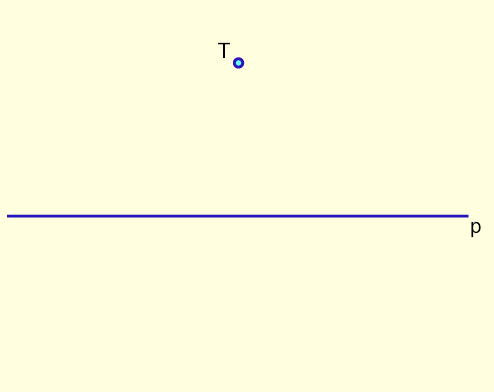
\includegraphics[width=50mm]{slike/fig-1.png}<1>
		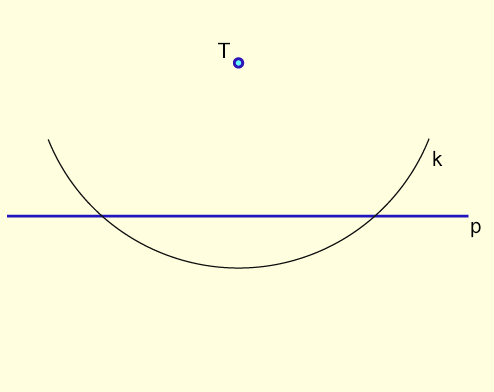
\includegraphics[width=50mm]{slike/fig-2.png}<2>
		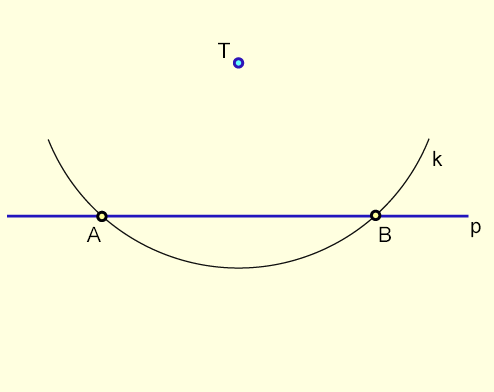
\includegraphics[width=50mm]{slike/fig-3.png}<3>
		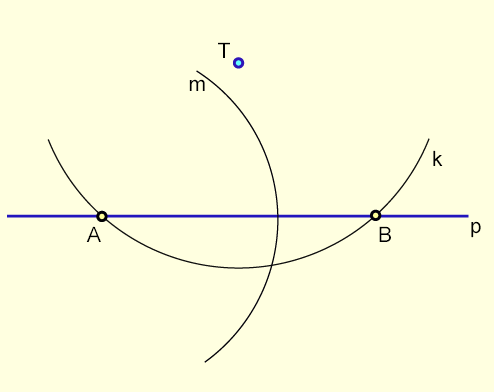
\includegraphics[width=50mm]{slike/fig-4.png}<4>
		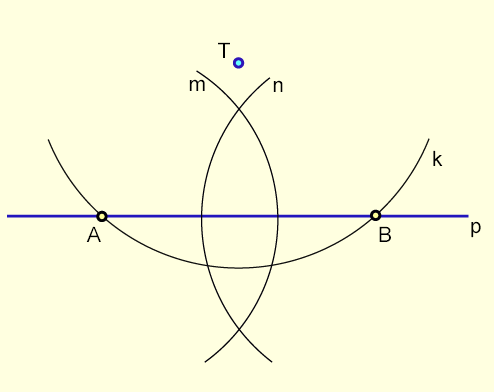
\includegraphics[width=50mm]{slike/fig-5.png}<5>
		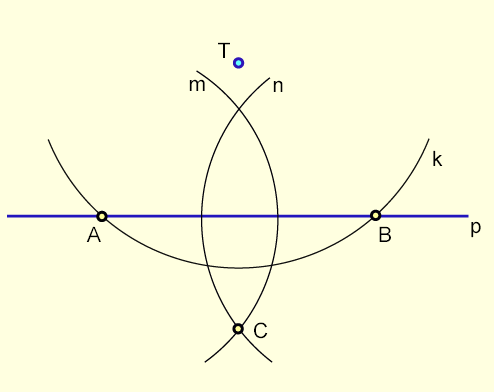
\includegraphics[width=50mm]{slike/fig-6.png}<6>
		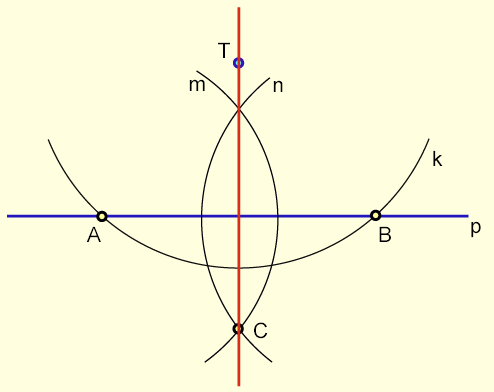
\includegraphics[width=50mm]{slike/fig-7.png}<7>
		\centering
	\end{columns}
\end{frame}

				% Spodnje je za nalogo 3.4.

				% % Sliko smo naredili tako, da so točke A, B, T in C vse enako oddaljene
				% % od presečišča premic; kot ATC je 45°.
				% % Vsi krožni loki imajo radij 2.
				% \tikzmath{
				% 	% Razdalja od točke T do premice p je tako 2*sin(45°).
				% 	\t = 2*sin(45);
				% 	% Razdalja začetka loka m do premice p
				% 	% oz. razdalja točke T' levo in zgoraj od točke T do premice
				% 	\tt = 2*sin(60);
				% 	% Razdalja točke T' od navpične premice skozi T
				% 	\td = \t-2*cos(60);
				% }
				% % Definicija točke T
				% \coordinate [label={[blue, above left]:$T$}] (T) at (0,{\t});
				% % Risanje točke T
				% \fill[blue] (T) circle (2pt);
				% % Premica p
				% \draw[blue, very thick] (-2,0) -- (2,0) node[right] {$p$};
				% \pause
				% % Definicija pomožne točke A' in risanje krožnega loka k, ki se začne v A'
				% \coordinate (A') at ({-\tt},{\td});
				% \draw[gray, thin] (A') arc[start angle=210, end angle=330, radius=2] node[right] {\scriptsize $k$};
				% \pause
				% % Točka A
				% \coordinate [label=below left:{\scriptsize $A$}] (A) at ({-\t},0);
				% \draw (A) circle (1.5pt);
				
				% % Naloga 3.4.1.: Narišite še točko B (skupaj z oznako)
				
				% % Naloga 3.4.2.: Definirajte točko T', v kateri se začne lok m in narišite lok m z oznako.
				% % Lok je definiran s točko, v kateri se lok začne (ne središče!), z začetnim in končnim kotom ter radijem.
				% % Koti so vedno podani enako: kot 0 je v smeri x osi in se veča v nasprotni smeri urinega kazalca.

				% % Naloga 3.4.3.: Definirajte točko T'' in narišite lok n z oznako.
				
				% % Naloga 3.4.4.: Definirajte in narišite točko C.

				% % Naloga 3.4.5.: Narišite premico skozi točki T in C.

				% Konec vsebine za nalogo 3.4.


% Naloga 4
% \begin{frame}{Graf funkcije s TikZ}
% 	\centering
% 	\begin{tikzpicture}
% 		\begin{axis}[
% 			axis lines = middle,
% 			domain = 0:10,
% 			width = 9cm,
% 			height = 8cm,
% 			xtick = {0, 1, 2, 3, 4, 5, 6, 7, 8},
% 			ytick = {0, 1, 2, 3, 4, 5, 6},
% 			ymin = -1,
% 			ymax = 7,
% 			grid = both
% 		]
% 		\end{axis}
% 	\end{tikzpicture}
% \end{frame}

\section{Paket \texttt{beamer} in tabele}

\section[Matematika, 2. del\\\large{Zaporedja, algebra, grupe}]{Matematika, 2. del}

\end{document}